\documentclass[tikz]{standalone}
\usepackage{fontawesome}
% Font
\usepackage{mathpazo}
\usepackage{libertine}
\renewcommand*\sfdefault{phv}

\large

% Color
\usepackage{xcolor}
\definecolor{f1}{HTML}{F39019}
\definecolor{b1}{HTML}{DE6A10}
\definecolor{f2}{HTML}{51A7F9}
\definecolor{b2}{HTML}{0365C0}
\definecolor{f3}{HTML}{70BF41}
\definecolor{b3}{HTML}{00882B}

% tikz
\usepackage{tikz}
\tikzstyle{every node}=[font=\sffamily]
\usetikzlibrary{shapes,arrows,positioning,calc,decorations.markings,backgrounds}
\tikzstyle{c1} = [thick,draw=b1,fill=f1]
\tikzstyle{c2} = [thick,draw=b2,fill=f2]
\tikzstyle{c3} = [thick,draw=b3,fill=f3]
\tikzstyle{cg} = [thick,draw=gray!50,fill=gray!30]
\tikzstyle{rect} = [rectangle, minimum height=1cm]
\tikzstyle{roundrect} = [rect, rounded corners=.2cm]
\tikzstyle{io} = [trapezium, trapezium left angle=70, trapezium right angle=110]
\tikzstyle{arrow} = [thick,->,>=stealth]

\tikzstyle{box} = [minimum width=18.6cm, minimum height=2cm,draw=gray!50, rounded corners, very thick]
\tikzstyle{title} = [font=\rmfamily \large, xshift=.3cm, yshift=.25cm,align =center, fill=white]
\tikzstyle{icon} = [minimum width=1cm, minimum height=1cm]
\tikzstyle{tag} = [minimum height=1cm]
\tikzstyle{ma} = [arrow, cg, line width=.2cm, shorten >=0.4cm,shorten <=.2cm]

\begin{document}
	
\begin{tikzpicture}[node distance=2cm]
\node (b1) [box] {};
\node (w1) [title, below=0 of b1.north west, anchor=north west] {\textbf{Chapter 3:} Exploring Temporal Relationship through User Annotations};
\node (icon11) [icon, below=0.2 of w1.south west, anchor=north west] {\faEdit};
\node (data1) [tag, right=0 of icon11] {User Annotations};
\node (icon12) [icon, right=6 of icon11.west, anchor=west] {\faHourglassHalf};
\node (dim1) [tag, right=0 of icon12] {Temporal};
\node (icon13) [icon, right=12 of icon11.west, anchor=west] {\faUserSecret};
\node (dom1) [tag, right=0 of icon13] {Intelligence Analysis};

\node (b2) [box, below=of b1] {};
\node (w2) [title, below=0 of b2.north west, anchor=north west]{\textbf{Chapter 4:} Visualizing Temporal and Thematic Relationships};
\node (icon11) [icon, below=0.2 of w2.south west, anchor=north west] {\faEdit};
\node (data1) [tag, right=0 of icon11] {Manual};
\node (icon12) [icon, right=6 of icon11.west, anchor=west] {\faHourglassHalf};
\node (dim1) [tag, right=0 of icon12] {Temporal};
\node (icon13) [icon, right=12 of icon11.west, anchor=west] {\faUserSecret};
\node (dom1) [tag, right=0 of icon13] {Intelligence Analysis};


\node (b3) [box, below=of b2] {};
\node (w3) [title, below=0 of b3.north west, anchor=north west]{\textbf{Chapter 5:} Analyzing the Sensemaking Process through Semi-Automatic Provenance Capture};
\node (icon11) [icon, below=0.2 of w3.south west, anchor=north west] {\faEdit};
\node (data1) [tag, right=0 of icon11] {Manual};
\node (icon12) [icon, right=6 of icon11.west, anchor=west] {\faHourglassHalf};
\node (dim1) [tag, right=0 of icon12] {Temporal};
\node (icon13) [icon, right=12 of icon11.west, anchor=west] {\faUserSecret};
\node (dom1) [tag, right=0 of icon13] {Intelligence Analysis};


\node (b4) [box, below=of b3] {};
\node (w4) [title, below=0 of b4.north west, anchor=north west] {\textbf{Chapter 6:}  Understanding High-level Reasoning through Semi-Automatic Provenance Capture};
\node (icon11) [icon, below=0.2 of w4.south west, anchor=north west] {\faEdit};
\node (data1) [tag, right=0 of icon11] {Manual};
\node (icon12) [icon, right=6 of icon11.west, anchor=west] {\faHourglassHalf};
\node (dim1) [tag, right=0 of icon12] {Temporal};
\node (icon13) [icon, right=12 of icon11.west, anchor=west] {\faUserSecret};
\node (dom1) [tag, right=0 of icon13] {Intelligence Analysis};


\draw [ma] (b1) -- (b2);
\draw [ma] (b2) -- (b3);
\draw [ma] (b3) -- (b4);

\end{tikzpicture}
	
\end{document}